\documentclass[12pt, titlepage]{article}
\usepackage{float}

\usepackage[legalpaper, portrait, margin=0.8in]{geometry}

\usepackage{longtable}
\usepackage{booktabs}
\usepackage{graphicx}
\usepackage{tabularx}
\usepackage{hyperref}
\hypersetup{
    colorlinks,
    citecolor=black,
    filecolor=black,
    linkcolor=red,
    urlcolor=blue
}
\usepackage[round]{natbib}

\title{SE 3XA3: Software Requirements Specification\\Sketchy Super Mario Bros}

\author{Team 1, Wario's Miners
		\\ Jason Nam and namy2
		\\ Kristine Uchendu and uchenduc
		\\ Rylan Sykes and sykesr
}

\date{\today}

%\input{../Comments}

\begin{document}

\maketitle

\pagenumbering{roman}
\tableofcontents
\listoftables
\listoffigures

\begin{table}[bp]
\caption{\bf Revision History}
\begin{tabularx}{\textwidth}{p{3cm}p{2cm}X}
\toprule {\bf Date} & {\bf Version} & {\bf Notes}\\
\midrule
Feb. 11th 2022 & 1.0 & Kristine's initial notes have been added.\\
Feb. 11th 2022 & 1.1 & The group has come together to add all of their parts.\\
\bottomrule
\end{tabularx}
\end{table}

\newpage

\pagenumbering{arabic}

\section{Project Drivers}

\subsection{The Purpose of the Project}
Initially released in 1985, Super Mario Brothers is a platform game that was originally developed for Nintendo arcades. The game is often named as one of the greatest video games of all time and has sold over 50 million copies worldwide. In the game, the player controls Mario (or potentially his brother Luigi, if in multiplayer mode) on his journey through the Mushroom Kingdom to save Princess Toadstool from Bowser. Mario and/or Luigi have to overcome hazards, such as living mushrooms (called Goombas) and pits, with the help of power-up items like the Super Mushroom, the Fire Flower and the Starman. There is currently no official desktop version of the original 16-bit game, but there is an open-source desktop game emulating it. The purpose of the Sketchy Super Mario Brothers project is as follows: we aspire to improve upon the existing 16-bit Super Mario Brothers for Desktop Game, to create a user-friendly and enjoyable game experience for players.

\subsection{The Stakeholders}
\subsubsection{The Client}
The clients for this project are the instructor, Dr. Bokhari, and the teaching assistants (Stephanie Koehl, Abdul Rab Mohammad, Oluwaseun Owojaiyo, and Veerash Palanichamy). All information about the project is received from them. This information includes deadlines for key milestones, best practices for documentation, feedback, and more.

\subsubsection{The Customers}
The targeted customers for the improved desktop version of Super Mario Bros., are fans of any of the many variations of the game, as well as people who are interested in learning how to play the game. The customers are also people that would be interested in downloading the game on their desktop and playing the game on their computer.

\subsubsection{Other Stakeholders}
Because the basis of this project is improving upon a medium-sized open source project, another group of stakeholders for this project are developers who decide to contribute to this project in the future. For future developers the documentation needs to be detailed, and the code needs to be well-structured. Another potential stakeholder is Nintendo, the gaming company that created the original game. We do not own the rights to characters or the idea of the game so monetizing it is not an option, and we must avoid breaking any and all copyright laws.

\subsection{Mandated Constraints}
	\begin{itemize}
		\item The project is due on April 12th.
		\item The TAs need to be able to run the project on their computer.
		\item Our project must be based on the chose open open-source project (mario-game).
		\item There is no budget for this project so any software that needs to be bought cannot be considered.
	\end{itemize}

\subsection{Naming Conventions and Terminology}
	\begin{itemize}
		\item SSMB - Sketchy Super Mario Bros
		\item GUI - Graphical User Interface
		\item UI - User Interface
		\item UX - User Experience
		\item FR - Functional Requirement
		\item NF - Non-functional Requirement
		\item UC - Use Case
		\item BE - Business Event
		\item TA - Teaching assistant
	\end{itemize}
\subsection{Relevant Facts and Assumptions}
\subsubsection{Facts}
	\begin{itemize}
		\item The original project has approximately 1600 lines of code
		\item The original open-source projects has not implemented certain features of the original game.
	\end{itemize}

\subsubsection{Assumptions}
\begin{itemize}
		\item The user has PC
		\item The user's PC can run Java
		\item The user has Gradle installed on their computer
	\end{itemize}

\section{Functional Requirements}

\subsection{The Scope of the Work and the Product}

The scope of the project is to design and implement a clone of the 16-bit Mario game originally created for the SNES game console. This is achieved through the use of various modern libraries which enable development on multiple platforms concurrently. The project will be developed through a series of deliverables spanning 4 months which include: design documents, requirements specification, testing plan, and proof of concepts. The purpose of the project will be to allow gamers to play the original game on modern hardware despite not having the original game console.

\subsubsection{The Context of the Work}

Refer to the context diagram below.

\begin{figure}[h]
\centering
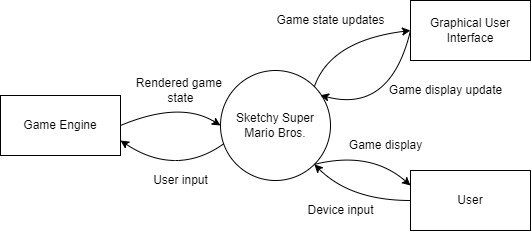
\includegraphics[scale=0.7]{images/contextdiagram.jpeg}
\caption{Context Diagram}
\end{figure}

\subsubsection{Work Partitioning}
\begin{table}[H]
\begin{tabular}{|p{0.1\linewidth}|p{0.2\linewidth}|l|p{0.4\linewidth}|}
\hline
\textbf{Business Event} & \textbf{Event Name}                      & \textbf{Input and Output}                                                             & \textbf{Summary}                                                                                        \\ \hline
BE1            & User enters game                & Game display (out)                                                           & Game will display the initial state (common amongst all starts)                                \\ \hline
BE2            & User exits game                 & Game display (out)                                                           & Game will exit, game state or display will not persist                                         \\ \hline
BE3            & User inputs movement action     & \begin{tabular}[c]{@{}l@{}}User input (in)\\ Game display (out)\end{tabular} & The GUI will display the corresponding action on the users device                              \\ \hline
BE4            & Mario contacts enemy            & \begin{tabular}[c]{@{}l@{}}Game state (in)\\ Game display (out)\end{tabular} & An attack from Mario (if done correctly) will kill an enemy                                    \\ \hline
BE5            & Enemy contacts Mario            & \begin{tabular}[c]{@{}l@{}}Game state (in)\\ Game display (out)\end{tabular} & Any contact from Mario (to enemy) that is non-lethal will result in Mario losing health points \\ \hline
BE6            & Mario takes damage              & \begin{tabular}[c]{@{}l@{}}Game state (in)\\ Game display (out)\end{tabular} & Mario will lose health accordingly and will be visibly displayed to the user                   \\ \hline
BE7            & Mario is eliminated             & \begin{tabular}[c]{@{}l@{}}Game state (in)\\ Game display (out)\end{tabular} & Mario's health points will reach 0 and game will display death messages                        \\ \hline
BE8            & Enemy is eliminated             & \begin{tabular}[c]{@{}l@{}}Game state (in)\\ Game display (out)\end{tabular} & Enemy will be cleared from game GUI and can no longer attack Mario                             \\ \hline
BE9            & Mario contacts powerup          & \begin{tabular}[c]{@{}l@{}}Game state (in)\\ Game display (out)\end{tabular} & Mario will visually and functionally react to the power-up obtained                            \\ \hline
BE10           & Mario falls off of platform      & Game display (out)                                                           & Game will display death message and restart                                                    \\ \hline
BE11           & Mario contacts brick from below & \begin{tabular}[c]{@{}l@{}}Game state (in)\\ Game display (out)\end{tabular} & Game will reward player based on Mario's state (power-up vs. no power-up)                      \\ \hline
BE12           & Mario contacts finish pole      & Game display (out)                                                           & Game is complete and game displays win screen, then restarts                                   \\ \hline
\end{tabular}
\end{table}


\subsubsection{Individual Product Use Cases}

The individual product use cases are equivalent to the events defined in the work partitioning.

% Please add the following required packages to your document preamble:
% \usepackage{longtable}
% Note: It may be necessary to compile the document several times to get a multi-page table to line up properly
\begin{longtable}{|l|p{0.2\linewidth}|p{0.5\linewidth}|}
\hline
\textbf{Use Case} & \textbf{Use Case Name}                   & \textbf{Summary}                                                                                        \\ \hline
\endfirsthead
%
\endhead
%
UC1      & User enters game                & Game will display the initial state (common amongst all starts)                                \\ \hline
UC2      & User exits game                 & Game will exit, game state or display will not persist                                         \\ \hline
UC3      & User inputs movement action     & The GUI will display the corresponding action on the users device                              \\ \hline
UC4      & Mario contacts enemy            & An attack from Mario (if done correctly) will kill an enemy                                    \\ \hline
UC5      & Enemy contacts Mario            & Any contact from Mario (to enemy) that is non-lethal will result in Mario losing health points \\ \hline
UC6      & Mario takes damage              & Mario will lose health accordingly and will be visibly displayed to the user                   \\ \hline
UC7      & Mario is eliminated             & Mario's health points will reach 0 and game will display death messages                        \\ \hline
UC8      & Enemy is eliminated             & Enemy will be cleared from game GUI and can no longer attack Mario                             \\ \hline
UC9      & Mario contacts powerup          & Mario will visually and functionally react to the power-up obtained                            \\ \hline
UC10     & Mario falls off of platform     & Game will display death message and restart                                                    \\ \hline
UC11     & Mario contacts brick from below & Game will reward player based on Mario's state (power-up vs. no power-up)                      \\ \hline
UC12     & Mario contacts finish pole      & Game is complete and game displays win screen, then restarts                                   \\ \hline
\end{longtable}

\subsection{Functional Requirements}

\begin{longtable}{|l|p{0.2\linewidth}|p{0.2\linewidth}|p{0.2\linewidth}|p{0.06\linewidth}|l|}
\hline
\textbf{FR} & \textbf{Requirement}                                                 & \textbf{Rationale}                                                                   & \textbf{Fit Criterion}                                                                              & \textbf{Use Case} & \textbf{Created} \\ \hline
\endfirsthead
%
\endhead
%
FR1         & The user must be able to start a new game                            & A new game must be started in order to play                                          & A new game is able to start                                                                         & UC1               & 2022-02-11       \\ \hline
FR2         & The user must be able to exit the game                               & The game must be able to exit for users to stop playing                              & The game is able to terminate                                                                       & UC2               & 2022-02-11       \\ \hline
FR3         & The user must be able to move Mario to the right and left            & Mario must move left and right as the game is a side scroller                        & Mario is able to move right and left depending on user input                                        & UC3               & 2022-02-11       \\ \hline
FR4         & The user must be able to move Mario up (jump)                        & There are platforms on higher levels that require jumping                            & Mario is able to jump                                                                               & UC3               & 2022-02-11       \\ \hline
FR5         & Mario, enemies, and power-ups in the game must be subject to gravity & Said objects should be able to jump and fall down, as well as descend from platforms & Said objects descend when mid-air                                                                   & UC3               & 2022-02-11       \\ \hline
FR6         & Mario must be able to attack enemies                                 & Mario can eliminate enemies for path-clearing as well as rewards                     & Mario can land on enemies to eliminate them                                                         & UC4, UC8          & 2022-02-11       \\ \hline
FR7         & Mario must be able to take damage from the environment and enemies   & User must face challenges when clearing the level                                    & Mario is able to lose health points                                                                 & UC5, UC6          & 2022-02-11       \\ \hline
FR8         & Mario must be able to be eliminated                                  & Game needs a way for the user to fail the level                                      & Mario reaches 0 health points                                                                       & UC7               & 2022-02-11       \\ \hline
FR9         & User must be visibly notified when Mario loses health points         & User should be aware that they are losing health points                              & Animation/re-color displays when Mario loses health points                                          & UC6               & 2022-02-11       \\ \hline
FR10        & Game must display a 'Game Over' screen when Mario is eliminated      & User should be aware that they have lost                                             & Message is displayed and game is restarted                                                          & UC7               & 2022-02-11       \\ \hline
FR11        & User must be visibly notified when enemy loses health points         & User should be aware that enemy has lost health points                               & Animation/re-color displays on enemy                                                                & UC4, UC8          & 2022-02-11       \\ \hline
FR12        & Enemies must be removed from display when eliminated                 & Indicates to user that enemy is eliminated                                           & Enemy no longer appears on GUI and is unable to interact with Mario                                 & UC8               & 2022-02-11       \\ \hline
FR13        & Mario must be able to consume power-ups                              & User must have a way to clear level easier                                           & Mario visibly consumes power-up and respective ability is visibly and functionally applied to Mario & UC9               & 2022-02-11       \\ \hline
FR14        & Mario must be able to break bricks                                   & Allows user to obtain coins                                                          & Coins will appear from bricks when Mario jumps and makes contact from brick from below until broken & UC11              & 2022-02-11       \\ \hline
FR15        & User must be able to finish level                                    & Allows user to complete game                                                         & Win screen must be displayed when Mario makes contact with Finish Pole                              & UC12              & 2022-02-11       \\ \hline
\end{longtable}

\section{Non-functional Requirements}

\subsection{Look and Feel Requirements}
\begin{itemize}
    
	\item[NF1] 
        Description: The system shall display intuitive GUI.
        
        Rationale: To allow users to get familiar with the interface quickly.
        
        Originator: Jason Nam
        
        Fit criterion: The users are able to select stages and set preferences within the options window within 1 minute of system use.
        
        Priority: High
        
        History: Created February 11, 2022
        
    \item[NF2]
        Description: The system shall look similar to the original Super Mario Bros 16 bit game.
        
        Rationale: To ensure that users who play this game will identify it as or as similar to the original Super Mario Bros 16 bit game.
        
        Originator: Jason Nam
        
        Fit criterion: By first playing this system, 80 percent of users will immediately identify the system as a Super Mario Bros game.
        
        Priority: Medium
        
        History: Created February 11, 2022
        
    \item[NF3]
        Description: The system shall appear nostalgic.
        
        Rationale: To ensure users who have enjoyed the original Super Mario Bros 16 bit will thoroughly enjoy this system.
        
        Originator: Jason Nam
        
        Fit criterion: The users who have memories of Super Mario Bros will stay on the system for more than 5 minutes.
        
        Priority: Medium
        
        History: Created February 11, 2022
        
\end{itemize}

\subsection{Usability and Humanity Requirements}

\begin{itemize}
    \item[NF4]
Description: The system shall be used by users with no knowledge about the system mechanics.

Rationale: To ensure that users who play this game for the first time will not struggle.

Originator: Jason Nam

Fit criterion: 50 percent of first time users will be able to pass the first stage.

Priority: Medium

History: Created February 11, 2022

    \item[NF5]
Description: The system shall be used by users with a simple understanding of the English language.

Rationale: To ensure that users will not require vast english vocabulary to understand system mechanics.

Originator: Jason Nam

Fit criterion: 30 percent of users will have a different native language other than english.

Priority: Low

History: Created February 11, 2022

    \item[NF6]
Description: The system shall use symbols and terms that are easy to understand.

Rationale: To avoid forcing users to learn new symbols and terms that can hinder their satisfaction with the system.

Originator: Jason Nam

Fit criterion: 90 percent of users will subconsciously identify symbols and terms used in the system.

Priority: Medium

History: Created February 11, 2022

    \item[NF7]
Description: The system shall be made usable by partially sighted users.

Rationale: To ensure users with partially disabled sights are able to enjoy the system without serious impairment.

Originator: Jason Nam

Fit criterion: Less than 20 percent of users with partially sighted disabilities will express severe discomfort with the system.

Priority: Medium

History: Created February 11, 2022

\end{itemize}

\subsection{Performance Requirements}

\begin{itemize}
    \item[NF8]
Description: The system shall be reliable with little to no failures.

Rationale: To ensure users can run the system without system failure.

Originator: Jason Nam

Fit criterion: The system will fail no less than 3 times in a day.

Priority: High

History: Created February 11, 2022

    \item[NF9]
Description: The system shall be available.

Rationale: To ensure users can install the system.

Originator: Jason Nam

Fit criterion: The system will not be available to install no less than 5 times a year.

Priority: Low

History: Created February 11, 2022

    \item[NF10]
Description: The system shall be responsive to user input and perform requested action if required criteria are met.

Rationale: To ensure user satisfaction is not disturbed by latency and wrong responses.

Originator: Jason Nam

Fit criterion: After user input, the system will respond within TIME\_RESPONSE with the requested action and response.

Priority: High

History: Created February 11, 2022
\end{itemize}

\subsection{Operational and Environmental Requirements}

\begin{itemize}
    \item[NF11]
Description: The system shall be portable on Linux systems.

Rationale: To allow users on Linux systems to run this system.

Originator: Jason Nam

Fit criterion: The system is Linux compatible.

Priority: Low

History: Created February 11, 2022

    \item[NF12]
Description: The system shall be portable on Windows systems.

Rationale: To allow users on Windows systems to run this system.

Originator: Jason Nam

Fit criterion: The system is Windows system compatible.

Priority: High

History: Created February 11, 2022

    \item[NF13]
Description: The system shall be programmed in a language that will be operable on future operating platforms.

Rationale: To ensure the system will be usable after future updates.

Originator: Jason Nam

Fit criterion: The system is written in a programming language that is cross-platform.

Priority: High

History: Created February 11, 2022

\end{itemize}

\subsection{Maintainability and Support Requirements}

\begin{itemize}
    \item[NF14]
Description: The system shall be easy to maintain.

Rationale: To ensure the maintainability of the system will be simple and costless.

Originator: Jason Nam

Fit criterion: The system takes less than 100 lines of code modification to maintain.

Priority: Medium

History: Created February 11, 2022

\end{itemize}

\subsection{Security Requirements}

\begin{itemize}
    \item[NF15]
Description: The system shall not collect and upload user data without authorization.

Rationale: To protect privacy of users and their personal information.

Originator: Jason Nam

Fit criterion: The system does not have any function that can collect and upload user data.

Priority: Low

History: Created February 11, 2022

\end{itemize}

\subsection{Cultural Requirements}

\begin{itemize}
    \item[NF16]
Description: The system shall not contain any imagery or text that could be regarded as hostile or offensive towards users and their cultures.

Rationale: Users will be unsatisfied due to the hostile or offensive context the game produces.

Originator: Jason Nam

Fit criterion: System does not contain any offensive cultural imagery or text.

Priority: Medium

History: Created February 11, 2022

\end{itemize}

\subsection{Health and Safety Requirements}

\begin{itemize}
    \item[NF17]
Description: The system shall avoid causing epileptic seizures to users, and avoid impairing user visions.

Rationale: To ensure the system does not cause epileptic seizures to users.

Originator: Jason Nam

Fit criterion: Less than 1 percent of users will express epileptic symptoms with the system.

Priority: High

History: Created February 11, 2022

\end{itemize}

\section{Project Issues}

\subsection{Open Issues}

A predominant issue is that the version of the libraries and package used in the original game are old and not compatible with newer versions of other software required to run the project. This prevents running the game and workarounds are still being looked into.


\subsection{Off-the-Shelf Solutions}

There are other open source 16-bit Mario clones existing on GitHub (and probably elsewhere).

\subsection{New Problems}

There are no new problems that are expected to arise.

\subsection{Tasks}
Refer to the Gantt chart below.
\begin{figure}[H]
    \centering
    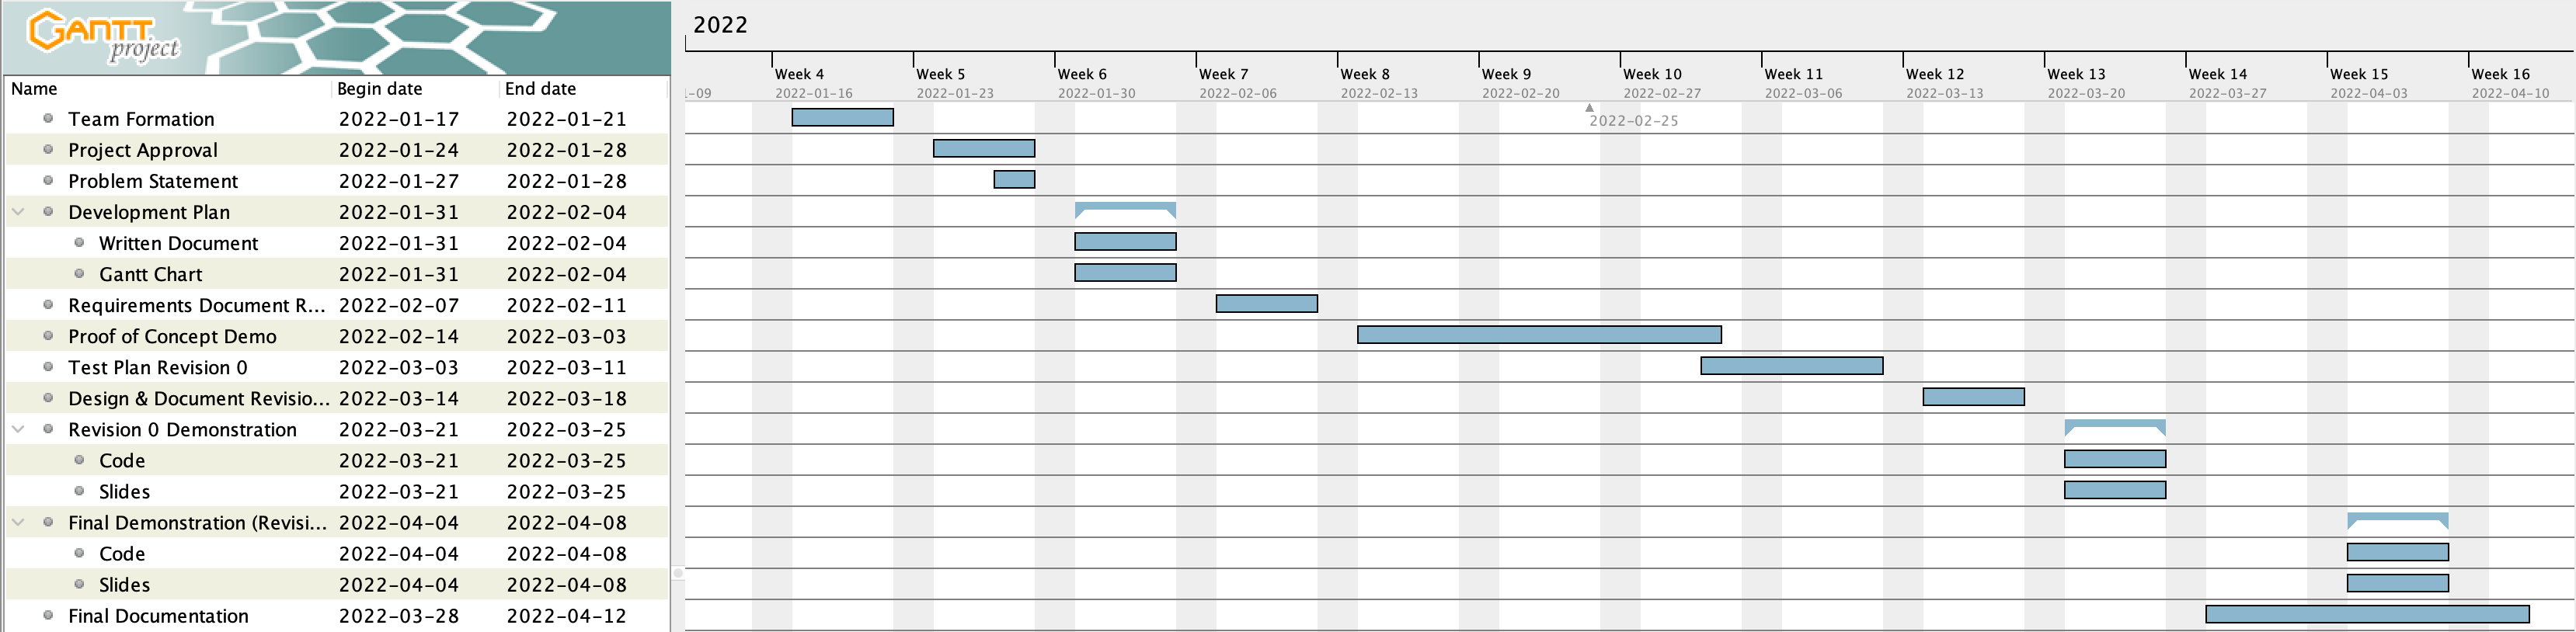
\includegraphics[scale=0.3]{images/Screen Shot 2022-02-11 at 8.50.38 PM.png}
    \caption{Gantt Chart.}
    \label{fig:my_label}
\end{figure}

\subsection{Migration to the New Product}

The new product will support newer versions of the original libraries that were built using the project.

\subsection{Risks}

The system is built on outdated versions of certain software, such as Gradle. This will hinder maintainability of the system. This will also hinder the ability to perform version control on the program.

\subsection{Costs}

There are no known costs for this project.

\subsection{User Documentation and Training}
\begin{itemize}
    \item \textbf{Download Instructions:} The first set of documentation needed for the user is a document explaining how the game is to be downloaded and how users must go about configuring and running the game.
    \item \textbf{Walk-Through Video:} If a player has never played the game before than providing a walk through video should help a new player understand the game's objectives.
    \item \textbf{Help Drop-down:} During game play, if a player forgets what the controls are, then they should be able to hover over a help icon that outlines what keys to uses on your keyboard, as well as what those keys do in the game.

\end{itemize}
\subsection{Waiting Room}
\begin{itemize}
    \item Create additional levels that matches levels from original game
    \item Create a special final level in which the objective is to defeat the final boss.
\end{itemize}

\subsection{Ideas for Solutions}
\begin{itemize}
    \item Utilize object oriented features of Java and graphics library libgdx and reference material from the original game
\end{itemize}

\bibliographystyle{plainnat}

\bibliography{SRS}

\newpage

\section{Appendix}

\subsection{Symbolic Parameters}

\begin{itemize}
    \item TIME\_RESPONSE - A time constant quantifying the amount of time it takes the system to respond to a user input.
\end{itemize}

\end{document}